%%%%%%%%%%%%%%%%%%%%%%%%%%%%%%%%%%%%%%%%%%%%%%%%%%%%%%%%%%%%%%%%%%%%%%%%
% Plantilla TFG/TFM
% Universidad de A Coruña. Facultad de Informática
% Realizado por: Welton Vieira dos Santos
% Modificado: Welton Vieira dos Santos
% Contacto: welton.dossantos@udc.es
%%%%%%%%%%%%%%%%%%%%%%%%%%%%%%%%%%%%%%%%%%%%%%%%%%%%%%%%%%%%%%%%%%%%%%%%


\chapter{Descripción del framework para el desarrollo de aplicaciones en robots autónomos ROS / ROS2 
}

\section{Introducción}
Robot Operating System (ROS) es un sistema muy utilizado en mundo de la investigación y desarrollo en el campo de la robótica debido a las facilidades y recursos con los que cuenta el desarrollador para sus proyectos.

Debido a su uso y evolución ha despertado el interes de grandes corporaciones del sector, como Amazon, Microsoft, Sony Corporation, etc. Las cuales tambien han aportado al desarrollo del propio sistema



\section{Historia}
ROS surge como el resultado de la ambición de dos estudiantes de doctorado, Eric Berger y Keenan Wyrobek, de la Universidad de Stanford por crear un sistema de referencia para proporcionar un punto de partida en el que empezar a construir a sus compañeros, los cuales tenían problemas y se veían limitados por la naturaleza tan diversa del mundo de la robótica.
\newpage

En un primer paso para ese sistema unificado, desarrollaron el PR1 (\href{https://robots.ieee.org/robots/pr1/}{\textit{Personal Robot 1}}) como un prototipo hardware sobre el que comenzar a trabajar en el software, tomando prestadas las mejores prácticas de otros marcos de desarrollo open source. En busca de financiación Berger y Wyrobek se encontraron con Scott Hassan, fundador de \href{https://www.businessinsider.com/a-look-back-at-willow-garage-2016-2}{\textit{Willow Garage}}, éste compartía la visión de un ``Linux para la robótica'' y así ROS se ganó el amparo del instituto de investigación y comenzó una nueva etapa en su desarrollo.

Willow Garage desarrollaría el PR2 (\href{https://www.xatakaciencia.com/robotica/pr2-el-robot-de-codigo-abierto}{\textit{Personal Robot 2}}) ya con ROS como software. Numerosos investigadores de diferentes instituciones contribuyeron a esta primera versión, convirtiendo a ROS en una plataforma multi-robot con un desarrollo descentralizado.

Actualmente, cada desarrollador puede desarrollar librerías nuevas para ROS y compartirlas con todos los miembros de la comunidad, permitiendo un desarrollo dinámico y retroalimentado. Hoy en día la comunidad de ROS está formada por miles y miles de usuarios alrededor del mundo, creando proyectos de nivel aficionado hasta grandes composiciones de sistemas complejos para la automatización industrial.

ROS2 surge en 2015 con el objetivo de paliar las limitaciones de ROS original. Está construido como un conjunto paralelo de paquetes que se pueden instalar e interoperar con ROS, de manera que ROS es independiente y sigue funcionando correctamente, siendo una buena opción, al ser una versión robusta, estable y funcional, para la gente que se está iniciando en este mundo.

\section{Qué es ROS}
ROS no es un sistema operativo en sí, a pesar de que su nombre indique lo contrario, sino un meta operating system, lo cual significa que asume que hay un sistema operativo subyacente que le servirá de apoyo para llevar a cabo sus tareas.

ROS proporciona servicios estándar de un sistema operativo tales como abstracción del hardware, control de dispositivos de bajo nivel, implementación de funcionalidad uso común como paso de mensajes entre procesos y mantenimiento de paquetes. Está basado en una arquitectura de grafos donde el procesado toma lugar en los nodos, que pueden comunicarse con los sensores, control, estados, planificadores y actuadores, entre otros recursos.


Es de código libre bajo licencia BSD, donde esa licencia permite la libertad para uso comercial y uso en la investigación.

ROS tiene compatibilidad asegurada para los sistemas operativos basados en Unix debido a su dependencia con las colecciones dependientes de software de código abierto.


El objetivo principal de ROS es unificar y facilitar el desarrollo de los robots. La definición que se presenta en el sitio oficial es la siguiente:

\href{http://wiki.ros.org/ROS/Introduction}{\textit{``ROS is an open-source, meta-operating system for your robot. It provides the services you would expect from an operating system, including hardware abstraction, low-level device control, implementation of commonly-used functionality, message-passing between processes, and package management. It also provides tools and libraries for obtaining, building, writing, and running code across multiple computers.''}}

Por lo que se confirma el hecho de que ROS no es un sistema operativo, sino que trabaja conjuntamente con ellos para prestar nuevos servicios. 
Un sistema operativo, a grandes rasgos, es un software que provee una interfaz entre aplicaciones y el hardware. Es el encargado de asignar diferentes recursos mediante ciertos algoritmos y proporciona una capa de seguridad manteniendo un registro de los roles de cada usuario.

Es necesario comprender qué son las libraries y los frameworks antes de poder comprender enteramente a qué se refiere el concepto de meta SO. Las libraries o librerías son esencialmente grupos de funciones que se utilizan muy a menudo, que han llegado a cierto nivel de popularidad como para justificar su empaquetado en archivos separados. Estas librerías también se utilizan para que el software sea más limpio y elegante, además de que nos aseguran que ese código que estamos ``reutilizando'' ya ha sido probado y comprobado por lo que reduce las posibilidades de errores si se decidiera implementar a parte. Esto no quiere decir que no se puedan construir librerías propias, aquí simplemente se hace referencia a librerías de uso común. Un framework, o marco de desarrollo, es, esencialmente, una colección de librerías que pueden utilizarse para el desarrollo de aplicaciones particulares.

Una API es una Interfaz de Programación de Aplicaciones (Application Programming Interface), si se tiene código y se quiere usar sin saber todo sobre ese código, se utilizan las APIs. Una API provee de una capa de abstracción y de acceso al código subyacente, lo cual es bastante útil cuando se trabaja en proyectos, ya que se puede utilizar código revisado y probado a fondo (librerías, marcos, …) sin tener que preocuparse del ‘cómo funcionará’.

Un meta sistema operativo tiene una gran cantidad de funcionalidades, tantas que no se puede categorizar dentro del mundillo de los marcos o los grupos de librerías pero no suficientes como para encasillarlo dentro de los sistemas operativos, por lo que ROS es tratado como un middleware, software que se sitúa entre el sistema operativo y las aplicaciones que se ejecutan en él.

Se podría concluir con que ROS es una colección de frameworks para el desarrollo de software de robots que, a pesar de no ser un sistema operativo, ofrece servicios estándar de estos como pueden ser la abstracción del hardware, el control de dispositivos de bajo nivel, el paso de mensajes entre procesos … Es importante destacar que ROS no es un lenguaje de programación, el hecho de que esté escrito en C++ no implica que la implementación de librerías en otros lenguajes como Python o Java no sea soportada.

\section{Objetivo de ROS}

ROS fue diseñado y pensando con la intención de que los usuarios pudieran elegir libremente las herramientas y bibliotecas que interactuaran con el núcleo de ROS y para que de esta forma sus usuarios pudieran cambiar sus desarrollos de software para adaptarse a su robot y área de aplicación. Como tal, hay muy poco que sea realmente esencial para ROS, más allá de la estructura general dentro de la cual los programas deben coexistir y comunicarse. En cierto sentido, ROS es el nexo subyacente detrás de los nodos y el paso de mensajes. Sin embargo, en realidad, ROS es mucho más que un aglomerado de bibliotecas. ROS es un conjunto rico de herramientas ademas de un amplio conjunto de capacidades proporcionadas por paquetes, como consecuencia resulta un ecosistema en constante crecimiento. 

\section{ROS2}

¿Por qué nació ROS2? La robótica, como muchos otros campos, está en continua evolución y ciertas limitaciones de ROS1 propiciaron la creación de ROS2 para adaptarse a la corriente actual del mundo de la robótica y a los nuevos requisitos. A continuación se comentan algunas de las diferencias más significativas entre ambos proyectos:

\begin{itemize}
    \item Una de las mayores diferencias es la desaparición del Master en ROS2, es decir, se deja atrás el modelo centralizado de ROS1, donde se debía inicializar un ROS master antes de correr un nodo y actuaba como DNS para los nodos de manera que se pudieran comunicar entre ellos, y se pasa a que, en ROS2, los propios nodos avisan al resto de su aparición en la red o de su marcha, cada nodo tiene la capacidad de descubrir otros nodos. Se puede iniciar un nodo sin necesidad de preocuparse de si hay un master corriendo o no, lo cual permite crear sistemas completamente distribuidos donde cada nodo es independiente y no está atado a un master global.
    \item ROS1 hacía uso de \href{http://wiki.ros.org/ROS/TCPROS}{TCPROS} el cual utiliza TCP/IP para el envío de los mensajes y la comunicación entre servicios, las conexiones entrantes se reciben a través de un socket de servidor TCP con un encabezado que contiene el tipo de datos del mensaje y la información del enrutamiento. En ROS2 se ha hecho el cambio a DDS (\href{https://design.ros2.org/articles/ros_on_dds.html}{Data Distribution Service}) el cual es un middleware\footnote{\textbf{Middleware o lógica de intercambio de información entre aplicaciones} (interlogical), o Agente Intermedio, es un software que asiste a una aplicación para interactuar o comunicarse con otras aplicaciones, o paquetes de programas, redes, hardware o sistemas operativos.} con una arquitectura publicador/suscriptor ideal para la necesidad de desarrollar aplicaciones en tiempo real. Aporta flexibilidad y aumenta el rendimiento al permitir la comunicación directa entre nodos y una alta capacidad de configuración gracias al Quality of Service, que son un conjunto de parámetros que controlan el comportamiento del sistema DDS, como pueden ser el consumo de recursos o la tolerancia a fallos.
    \item Lenguajes de programación: ROS1 trabaja mayoritariamente con Python2.7 y C++1 (aunque la última versión de ROS1 ha realizado el salto a Python3), ROS2 permite trabajar en lenguajes más actualizados como Python3.5 y versiones superiores de C++, sin dejar de dar soporte para otros lenguajes.
    \item Sistemas operativos: si bien ROS1 ya da soporte a Linux y MacOs (distribuciones basadas en UNIX), ROS2 dio el salto al Windows 10 aunque aún se encuentra en fases experimentales
\end{itemize}


Hoy en día ROS1: \href{http://wiki.ros.org/noetic}{ROS Noetic Ninjemys} es la última versión de ROS1. El objetivo principal de esta versión final de ROS1 es proporcionar soporte para Python3 de manera que los desarrolladores, instituciones y organizaciones que necesiten continuar trabajando con ROS1 puedan seguir haciéndolo durante un tiempo. Pero la fecha de fin de vida prevista para ROS Noetic está para 2025, es decir, el fin de ROS1 se acerca.

Para ROS2, a partir de la versión \href{https://docs.ros.org/en/foxy/Releases/Release-Foxy-Fitzroy.html}{Foxy Fitzroy} (ref) se está lanzando una nueva versión cada año, siendo la más reciente de todas \href{https://docs.ros.org/en/foxy/Releases/Release-Galactic-Geochelone.html}{ROS2 Galactic Geochelone}, como ya se hizo anteriormente con ROS1.

¿Cuándo cambiar de ROS1 a ROS2? Esta pregunta no tiene fácil respuesta, ROS1 es todavía una versión fuerte, robusta y estable, con grandes cantidades de plugins desarrollados por terceros y una extendida documentación y, aunque eventualmente se acabará, aún le quedan ciertos años de vida útil.

Es probable que los usuarios nuevos de ROS deban comenzar aprendiendo ROS1 para así entender mejor ciertas características de ROS2, pero haciendo énfasis en migrar a ROS2 lo antes posible. ROS1 hoy en día es también una versión más. También es posible que ciertas herramientas y paquetes aún se hayan trasladado a ROS2, por lo que los usuarios que quieran hacer uso de estas utilidades no tendrán otra opción que usar ROS1, en estos casos el paquete \textit{ros1\_bridge} será interesante y conveniente.

Los usuarios más versados en ROS que desean comenzar un nuevo proyecto deberían seguir el camino de ROS2, de manera que haya que realizar menos trabajo de transiciones en el futuro. Los conceptos básicos entre ROS1 y ROS2 son muy similares, por lo que cuanta más experiencia en ROS1, menos tiempo tardarán en aprender ROS2.

En el caso de tener ya un código estable, una base en ROS1, para uno o más robots, o, incluso, para una organización en la que participen más desarrolladores, cambiar a ROS2 puede representar un desafío y causar más problemas de los que soluciona. Cuanto mayor sea la dimensión del código y la influencia de ROS en el proyecto en general, el cambio de versión requerirá más tiempo y será más y más complejo, una solución es seguir trabajando en ROS1 en estos proyectos ``legacy'' o heredados, y utilizar ROS2 como la versión para los proyectos nuevos. Si, sin embargo, se desea realizar el cambio es importante que las funciones que se necesiten estén ya implementadas en ROS2 y, en todo caso, utilizar \textit{ros1\_bridge} como apoyo durante la transición.

Tras haberlo mencionado un par de veces, es importante destacar la utilidad del paquete \href{https://github.com/ros2/ros1_bridge}{\textit{ros1\_bridge}} como una herramienta útil en este período de transición entre ROS1 y ROS2. Cuando se necesite trabajar con una base de código ROS1 ya existente pero se desea empezar a realizar funciones y funcionalidades nuevas en ROS2, se utiliza este paquete que, como su propio nombre indica, no es más que un puente entre las comunicaciones de ROS1 y ROS2. Aunque los conceptos entre ROS1 y ROS2 son los mismos, la comunicación subyacente no es compatible (directamente) y requiere cierta adaptación, aquí es donde entra en acción \textit{ros1\_bridge}.

Al hacer una transición a ROS2, se puede empezar portando algunos paquetes en ROS2 y hacer que estos paquetes comiencen a comunicarse con el resto de la aplicación en ROS1 y así sucesivamente, se portan tantos paquetes como sea necesario para que no quede nada escrito con ROS1, manteniendo la aplicación o proyecto operativos y funcionando de la manera esperada mientras se realiza el cambio.

\section{Arquitectura}

ROS esta dividido en dos partes básicas, una parte del sistema operativo y la otra a suite de paquetes aportados por la comunidad que implementan las funcionalidades como localización, mapeo simultáneo, planificación, percepción, simulación entre otros. En la imagen de la izquierda de la Figura \ref{fig:Estructura} muestra el ejemplo más amplio de la estructura de ROS.

\begin{figure}[H]
	\centering
	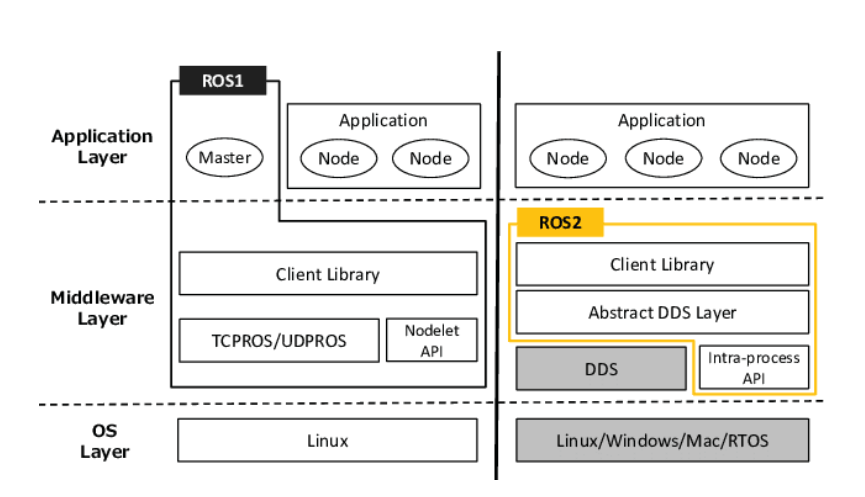
\includegraphics[scale=0.75]{imagenes/Estructura.png}
	\caption{\label{fig:Estructura}Estructura de las capas de ROS/ROS2}
\end{figure}

Como se puede observar, los procesos de ROS/ROS2 se representan como nodos, conocido como \textbf{ROS NODES} en una estructura gráfica, conectada por bordes llamados \textbf{ROS Topics}. Los ROS NODES pueden pasar mensajes entre si a través de los ROS Topics, en realizar llamadas de servicio a otros nodos, proporciona un servicio para otros nodos como recuperar y establecer datos compartidos de una base de datos común conocida como \textbf{Paramter Server}.

Un proceso llamado ROS Master hace que todo el proceso de control de los nodos sea prosible al registrar nodos para si mismo.

Los mensajes y las llamadas de servicio no son controlados por el MASTER, sino que el MASTER establece la comunicación entre pares y entre todos los procesos de nodo y después de que estos se registren con el MASTER. Esta arquitectura descentralizada ayuda bastante para trabajar con los robots, que a menudo consisten en un subconjunto de hardware informático en red, y pueden comunicarse con computadoras externas para realizar cálculos complejos

\section{Herramientas}
Las funcionalidades de ROS se espanden bastante con una variedad de herramientas que permiten los desarrolladores y investigadores visualizar, recompilar infomación y navegar de forma muy sencilla dentro de la estructura de paquetes que posee ROS. 

Se pueden crear código fuentes robustos para automatizar tareas muy complejas y otros procesos de configuración dentro de ROS. Con todo esas facilidades, ROS se torna una herramienta muy potente a la hora de hacer desarrollo para el campo de la robótica. 

La mayoría de las herramientas que provee ROS, las más importantes son:
\begin{itemize}
    \item \textbf{rosbash:} Es una herramienta que aumenta las funcionalidades del bash, funciona como un ZSH o otro sistema de terminal incorporado en ambiente Unix.
    \item \textbf{rviz:} Es una herramienta de simulación y visualización 3D para robots que es el entorno que se desenvolve los robots además de blindar información de los sensores, que son altamente configurables.
    \item \textbf{rosbag:} rosbag es una herramienta de línea de comandos para grabar y reproducir datos de mensajes y comunicaciones dentro de ROS. rosbag utiliza un formato de archivo llamado bags, que registra los mensajes de ROS mediante escuchar los ROS topic y almacena los mensajes en la medida que son emitidos. Visualizar los mensajes desde bag es mayormente lo mismo que tener los ROS Nodes originales reproduciendo estos mensajes. Esto hace de bags una herramienta muy útil para capturar la información que posteriormente se puede utilizar, analizar y posteriormente ser usada para el desarrollo de paquetes ROS por ejemplo. Mientas rosbag es una herramienta puramente de línea de comando, también posee una implementación rqt llamada \textit{rqt\_bag} que brinda una interfaces gráfica.
    \item \textbf{catkin:} catkin es la herramienta actual de compilación de ROS, habiendo reemplazado a rosbuild. catkin esta basada en CMake, es multiplataforma, de código abierto e independiente del lenguaje de programación.
    \item \textbf{roslaunch:} roslaunch es una herramienta usada para ejecutar múltiples nodos ROS de forma local o remota, de igual forma es usado para configurar parámetros en un servidor de parámetros ROS. Los archivos de configuración roslaunch, cuyo código esta escrito usando XML pueden de forma sencilla automatizar complejos procesos de arranque y configuraciones con un sólo comando. Las secuencias de comandos dentro de archivos roslaunch pueden anidar dentro de ellas llamadas a otras secuencias de comandos roslaunch, inicio de nodos ROS en máquinas específicas y hasta reiniciar procesos que se han caído.
\end{itemize}

\section{Conclusión}

De todas las características vistas hasta ahora sobre ROS/ROS2 no hay duda que se trata de una herramienta muy potente para trabajar con la robótica propiciando al investigador o desarrollador recursos impresionantes. Además de tener un costo bajo.
